%-------------------------------------------------------------------------------
\documentclass[11pt]{article}

\usepackage{booktabs}
\usepackage[usenames, dvipsnames]{color} 
\usepackage{dsfont}
\usepackage{epigraph}
\usepackage{graphicx}
\usepackage{hyperref}
\usepackage[utf8]{inputenc}
\usepackage{lscape}
\usepackage{natbib}
\usepackage{setspace}


\bibpunct{(}{)}{;}{a}{,}{,}

\setlength\topmargin{-0.375in}
\setlength\textheight{8.8in}
\setlength\textwidth{5.8in}
\setlength\oddsidemargin{0.4in}
\setlength\evensidemargin{-0.5in}
\setlength\parindent{0.25in}
\setlength\parskip{0.25in}

\hypersetup{                                                                                                    
    colorlinks=true,   
    linkcolor=BlueViolet,
    citecolor=BlueViolet,
    filecolor=BlueViolet,
    urlcolor=BlueViolet
}  

%-------------------------------------------------------------------------------

\title{{\bf\Large{\textsl{Maternal Mortality and Female Life Expectancy: }\\ 
\large\normalsize The Importance of Gender Inequality}} \footnotemark[7] 
\author{Sonia Bhalotra\\ \normalsize{University of Essex}\footnotemark[1] 
\and Damian Clarke\\ \normalsize{University of Oxford}\footnotemark[2]\\ 
\and Joseph Gomes\\ \normalsize{University of Essex}\footnotemark[3]\\\\ 
\and Atheendar Venkataramani\\ \normalsize{Massachusetts General Hospital}\footnotemark[4]\\}}

\date{\today}
\renewcommand{\thefootnote}{\fnsymbol{footnote}}

\footnotetext[1]{\noindent ISER \& Department of Economics, University of Essex, 
Wivenhoe Park, Colchster CO4 3SQ, United Kingdom, \texttt{e-mail: srbhal@essex.ac.uk}}


\footnotetext[2]{Department of Economics, University of Oxford, United Kingdom 
\texttt{ e-mail:damian.clarke@economics.ox.ac.uk}}

\footnotetext[3]{\noindent ISER, University of Essex, Wivenhoe Park, Colchster 
CO4 3SQ, United Kingdom, \texttt{ e-mail:jgomes@essex.ac.uk}}

\footnotetext[4]{Masachusstes General Hospital, USA 
\texttt{ e-mail:avenkataramani@partners.org} \\ \vspace{0.1cm} } 

\footnotetext[7]{We are grateful to all seminar participants in the FRG seminar 
at ISER, Essex, NEUDC 2014 conference in Boston University,  Growth Conference 
in ISI Delhi Dec 2014, and RES 2015 in Manchester, for their comments and 
feedback.}


%-------------------------------------------------------------------------------





\begin{document}
\thispagestyle{empty}
\maketitle
\renewcommand{\thefootnote}{\arabic{footnote}} \setcounter{footnote}{0} 



\begin{abstract}
Societies with higher levels of gender inequality are slower and less likely to
address women-specific health outcomes.  We demonstrate this by examining 
maternal mortality ratios (MMR) and the life expectancy gap which exists between
women and men.  We show that socities which are more gender predjudiced 
have higher levels of maternal mortality, slower rates of reduction of maternal 
mortality, and life expectancy differentials \emph{less} favourable for women.
This holds conditional on country income.  In terms of maternal mortality 
reductions, a 1 standard deviation (sd) reduction in gender predjudice is 
equivalent to a xx.xx-xx.xx sd increase in log(GDP).  Despite these large effects
on women's health, our various measures of gender predjudice are shown to have 
no significant effect on TB infection rates---a gender neutral illness which we 
consider as a placebo test.
\end{abstract}

\emph{JEL codes:} X00, X00, X00, X00.

\thispagestyle{empty}
\setlength{\baselineskip}{1.4\baselineskip} 
\newpage 
\begin{spacing}{1.4}

\section{Introduction}
\epigraph{`\textit{`In some regions of the world inequality between women and men 
directly involves matters of life and death, and takes the brutal form of unusually 
high mortality rates for women...}'' }{\citet{sen2001many}}


\section{Data and Descriptive Statistics}



\section{Methodology}
\label{scn:methodology}
\subsection{Gender Preferences and Women's Health}
We test our prevailing hypothesis that gender-biased preferences drive female-%
specific health outcomes.  To do so, we begin by estimating the following 
regression using the panel data described in the previous section:
\begin{equation}
\label{eqn:panel}
FemaleHealth_{it} = \alpha + \beta GenderBias_{it} + \gamma_i + \delta_t + 
               (\phi_i\times t) + \theta X_{it} + \varepsilon_{it}.
\end{equation}
Here $FemaleHealth_{it}$ is a measure of health stocks or outcomes speficic 
to women in country $i$ and time $t$.  As discussed in section X.X,
female health is measured in two ways: using a female-specific mortality measure
(MMR), and using a relative measure of female health stocks to male health stocks 
(LE advantage).  We include country-specific fixed effects $\gamma$, and year 
specific fixed effects $\delta$ while allowing for differential trends in female 
health measures by country.  Standard errors are always clustered at the level
of the country.

Consistent estimates of $\beta$---the effect of gender-biased preferences on
female health---requires that the transitory error term $\varepsilon_{it}$
contains no factors correlated with both our measure of gender bias and female 
health outcomes.  While in our most demanding specifications we include a 
number of time-varying controls $X_{it}$ (including levels and growth of GDP), 
it is unlikely that observable 
measures will capture all time varying country-specific factors which affect
both variables.  As such, we view (\ref{eqn:panel}) as compelling descriptive 
evidence, and later employ a number of alternative specifications, methodologies 
and falsification tests which allow us to reach causal conclusions regarding the 
effect of gender bias on female health.  We describe these tests in the following 
sections 

\subsubsection{Measuring Gender Bias}
\label{ssscn:gendbias}
In our most na\"ive regressions, we use a range of accepted measures of gender
bias as our independent variable in (\ref{eqn:panel}).  Different measures are 
collected at the level of the individual, or the level of the country, and in
each case, vary over time and space.  These initial variables are: desired sex
ratio; the Cingranelli et al.\ political, economic and social rights of women
measures; and proportional representation of women in national parliaments. We
provide additional descriptive statistics and discussion of these variables in 
section XX.

In each case we progressively control for $\log($GDP$)$, and an interaction 
between $\log($GDP$)$ and our independent variable of interest.  We thus 
estimate the effect of gender bias on woman-specific health outcomes conditional 
and unconditional on country income levels, to allay concerns that both gender 
bias and outcomes such as MMR are jointly driven by country income.

%-------------------------------------------------------------------------------
\subsubsection{Predetermined Measures of Gender Bias}
\label{ssscn:language}
Measures of gender bias used in estimation up to this point are (either directly 
or indirectly) based on contemporaneous decisions by a society and/or its 
members.  Thus, even controlling for time-varying covariates, trends and fixed 
effects, endogeneity concerns still exist.  Given these concerns, we focus on a 
measure of gender attitudes which is entirely pre-determined, and arguably 
entirely exogenous when considering contemporaneous maternal mortality and life 
expectancy advantage.

Following Givati and Troiano (2012) and Gay et al.\ (2013), we use measures of
the inherent gender neutrality (or gender bias) built into the grammatical 
structure of different languages.\footnote{These authors suggest that grammatical 
gender can influence and reflect gender attitudes in society and are correlated 
with different gender outcomes including maternity leave policy differences 
across countries (Givati and Troiano, 2012), female labour force participation, 
and political 
participation (Gay et al., 2013). Language grammar was established centuries in 
the past and is one of the features of language that is stable over long periods 
of time. Moreover, grammatical gender is something that an individual is born 
in to and thus arguably a more exogenous measure of gender bias in society.}  We 
estimate:
\begin{equation}
\label{eqn:gii}
FemaleHealth_{it} = \beta_0 + \beta_1 GII_i + \beta_2 PercentLang_i + X_{it} + X_i 
                  + \nu_{it},
\end{equation}
where $FemaleHealth_{it}$ is identical to that described in model 
(\ref{eqn:panel}). Here, $GII$, (Gender Intensity Index), refers to the measure 
of the gender bias inherent in the language, as coded by Givati and Troiano, and 
Gay et al.  Precise details regarding this variable are provided in section X.X 
and appendix X).

Given that the language of country $i$ is essentially fixed over time, we can no
longer include country fixed effects, as these capture (among other things) the
language spoken in the country.  We thus now control for both fixed ($X_{i}$) 
and time varying ($X_{it}$) country-level variables, including decade dummies, 
continent dummies, $\log($GDP$)$, the log of population, religion, income and 
climate factors.  Finally, given that $GII$ is defined based on the majority
language in each country, we control for the percentage of inhabitants of each
country which speak the particular language.

\subsubsection{Falsification Tests: Gender Neutral Disease Burden}
\label{ssscn:TB}
The analysis discussed so far in this section tests the hypothesis that gender
biased preferences slow the improvement of female-specific health outcomes 
(namely maternal mortality, and relative life expectancy).  In order to provide
evidence that it is indeed \emph{female}-specific health outcomes which are 
driven by gender preferences, we run a series of falsification tests.  These
falsification tests consist of estimating the previous regressions, however 
focusing on a gender-neutral health outcome.

We thus focus on rates of tuberculosis (TB) infection.  TB is a gender-neutral
condition\footnote{According to the WHO ``In most of the world, more men than 
women are diagnosed with tuberculosis (TB) and die from it. TB is nevertheless 
a leading infectious cause of death among women.''}, %http://www.who.int/tb/challenges/gender/en/
 and was the second most common infectious cause of death world wide in 2014 
(WHO, 2015). %http://www.who.int/mediacentre/factsheets/fs104/en/
Given that it affects individuals indiscriminately by gender, it is a
 particularly suitable placebo for our analysis.  Based on this placebo, we 
estimate analogues to (\ref{eqn:panel}) and (\ref{eqn:gii}).  For example, for 
(\ref{eqn:panel}) we estimate:
\begin{equation}
TB_{it} = \alpha^{TB} + \beta^{TB} GenderBias_{it} + \gamma^{TB}_i + \delta^{TB}_t + 
               (\phi^{TB}_i\times t) + \theta^{TB} X_{it} + \varepsilon^{TB}_{it},
\end{equation}
and if $\hat\beta$ but not $\hat\beta^{TB}$ is significantly (and economically)
significant, this lends support to the hypothesis that gender preferences halt
progress on (only) woman-specific conditions.


\subsection{Testing Mechanisms}
After documenting the effect that gender-biased preferences have on female
health outcomes, we turn to testing the mechanisms that drive these results.
Using the arrival of sulfanide drugs (the first antibiotics) to the United 
States in 1937, we test whether states which were early to legislate suffrage 
were more likely to adopt medical technologies which could be employed to 
directly reduce rates of maternal mortality. We define early legislators of 
suffrage as those states which passed suffrage laws prior to the mandated 
national reform in 1920.  Using these two groups of states, we follow 
Jayachandran et al.\ (2010) and estimate the following difference-in-differences 
specification around the 1937 date of arrival of sulf drugs:
\begin{eqnarray}
\label{eqn:sulfa}
log(MMR)_{st} & = \alpha + \beta \mathds{1}[Post1937]_t + \gamma(EarlySuf_{s}\times t)
                + \delta_1 (EarlySuf\times Post1937_t) \nonumber \\
              & + \delta_2 (EarlySuf\times Post1937_t\times t) + \phi_t + \mu_s
                + \upsilon_{st}.
\end{eqnarray}
In these regressions we always weight states ($s$) by their population, and 
cluster standard errors at the level of the state.

By estimating (\ref{eqn:sulfa}), we are able to split the quantitatively 
important (exogenous) 
reduction in maternal deaths which occurred with the arrival of the first 
antibiotics into three components.  The first, $\beta$, identifies the immediate 
general effect of sulfanide drugs on MMR, while $\delta_1$ and $\delta_2$ test 
whether there are larger level and trend breaks (respectively) in states that 
were early adopters of women's suffrage, and which presumably had long-standing 
norms evolving in favor of women's autonomy.

Sulfa drugs were also important in reducing morbidity and mortality from 
pneumonia.  Unlike maternal mortality, pneumonia mortality affects males 
more than females, and infants in particular.  Thus, as in section 
\ref{ssscn:TB}, we employ a similar logic, and use rates of pneumonia (for 
which there is also a post-1937 trend break), as a falsification test.  We 
restimate (\ref{eqn:sulfa}), replacing maternal mortality with pneumonia 
mortality as our dependent variable.  Our placebo test is based on the 
coefficients $\delta_1$ and $\delta_2$.  If states with a lower preference for 
female equality invest less (only) in applying available technologies to 
female-specific illnesses, then $\delta_1$ and $\delta_2$ should be negative in 
(\ref{eqn:sulfa}), but not significant in the gender-neutral pneumonia version
of (\ref{eqn:sulfa}) estimated for pneumonia rather than MMR.


\section{Results}




\subsection{US Case Study: Early Suffrage, Adoption of Medical 
Technology, and Maternal Mortality}
This supplement explores the interplay between early suffrage and the post-1937 fall in maternal mortality driven by the arrival of the first antibiotics in the United States. Women's suffrage was institutionalized at the national level in 1920 with the 19th amendment to the U.S. Constitution. However, prior to this, individual states had the authority to legislate women's suffrage with respect to state and local elections. About 40\% of U.S. passed suffrage laws prior to 1920. 

The evolution of women's suffrage is chronicled in \citet{miller2008women}. He contends, based on work by other scholars, that early adoption of women's suffrage was driven by slowly changing social norms with respect to role of women.\footnote{E.g. ``The most obvious pattern is geographic – all else equal, women in western states could vote before women elsewhere in America. Some historians suggest that frontier conditions were amenable to women’s suffrage because women supported restrictions on common western vices (drunkenness, gambling, and prostitution) or because the harsh realities of frontier life made it impossible to maintain traditional gender roles (Brown 1958; Grimes 1967).7 Many others argue that idiosyncratic circumstances in each state resulted in the vote for women (Larson 1971; Beeton 1986), citing rich historical evidence in support of this view.8 Quantitative studies yield strikingly inconclusive results (Cornwall, Dahlin, King, and Schiffman 2004). The single robust correlate of suffrage law enactment emerging from these studies is the share of women working in non-agricultural occupations (King, Cornwall, and Dahlin 2005). Although this presumably reflects changing social norms about the role of women, it evolved very gradually over time (Smith and Ward 1985; Goldin 1990) and can be distinguished econometrically from abrupt year-to-year legislative changes governing women’s right to vote.'' }  

The role of sulfa drugs in inducing a historic decline in maternal mortality is chronicled in \citet{jayachandran2008mortality}. Basically, log(MMR) was constant for a long period of time until 1937, when sulfa drugs were rapidly adopted in hospital and outpatient settings. Sulfa drugs were also important in reducing morbidity and mortality from pneumonia, as well. 

Following the main paper, it is worthwhile to ask if states adopting early women's suffrage, which presumably had long standing norms evolving in favor of women's autonomy gained more from the arrival of antibiotics than their later suffrage counterparts. We will look at both maternal mortality, the condition of interest, and pneumonia mortality, which affected males more than females, and infants in particular. The graphs below show that the gap between early (anytime before 1920) and late (laws passed in 1920) suffrage adopters for MMR widened after the arrival for sulfa drugs, but not so for pneumonia mortality:


We can verify this econometrically using state level mortality and suffrage data from the above papers. Basically, for the 1925-1943 time period, we can regress logged MMR against a linear year trend, a dummy = 1 for year = 1937 or later, and their interaction. These RHS variables can additionally be interacted with an indicator for early suffrage = 1, so as to assess whether the level and trend breaks are larger for these states. This specification follows that used in the aforementioned \citet{jayachandran2008mortality} study. As a falsification, we will do the same for logged pneumonia mortality. All models include state fixed effects, cluster S.E. at the state level, and weight observations (state-level) by their population:

Early suffrage states had significantly larger trend and level breaks for maternal mortality. However, for pneumonia mortality (for which there is a trend break only), we do not see any difference in the ``sulfa effect.''

The results suggest that preferences correlated with female suffrage may have influenced the specific adoption of medical technology for a ``women specific issue.''


In order to examine the parallel trend assumptions underlying our double-difference specification more 
completely, we plot event studies figures for both causes of death.  These event studies follow the 
specification in table \ref{MMRPneumSulfa}, however now fully interact early suffrage states with each year dummy.  This 
allows us to plot the difference between early- and late-suffrage states by year, both preceding, and after 
the sulfa reforms.  If the parallel trend assumptions hold, so that the only difference between the two types
of states arises after the date of the reform, we should see that all estimates plotted prior to the reform 
are not statistically distinguishable from zero.  What's more, if early suffrage states only make additional 
inroads in \emph{female} specific causes, we should see that all coefficients are insignificant for infant 
pneumonia, but post-reform coefficients \emph{are} significant for MMR.

This is precisely what we observe in figures  \ref{eventMMR} and  \ref{eventIPR}.  In figure 7 we see that all confidence intervals
include 0 prior to the reform, however in the year of the arrival of sulfa, and in the post-reform years, 
early suffrage states make significant improvements in MMR indicators when compared with their 
late-suffrage counterparts.  This suggests that prior to the reform, in the absence of sulfanid drugs, 
rates of maternal mortality evolved on a similar trajectory in both states, while in post-reform years, early 
suffrage states employ the available technology more effectively to address female-specific mortality 
causes.

When compared to figure \ref{eventIPR}, the contrast is stark.  With the exception of 1 in 18 years, there is no 
significant difference between the early- and the late-suffrage states in their trends in pneumonia 
death rates.  Fundamentally, as suggested in figure 6b, both states are equally able to leverage the 
arrival of sulfa drugs to reduce the gender-neutral (or indeed slightly male-biased) disease burden. This 
reinforces the idea discussed above that there are important differences in the way that more 
gender-biased states are able to employ health care technology to all, and to female-speficic, health 
outcomes.


\section{Conclusion}

Preventable maternal mortality is still very high in many developing countries, even after falling by almost 50\% since 1990 to the present day. Moreover, while IMR has been falling steadily in the last few decades, MMR rates started to fall only in the 1990s after initial stagnation. In this paper we show that MMR is a woman specific condition and differences in MMR and female life expectancy advantage across countries are a reflection of differences in gender attitudes across countries. 

We find that regardless of the measures of gender bias or woman's status in society we use including the stated son preference of mothers, women's political rights or the gender intensity of language grammar, we consistently find that  that cross country differences in gender inequalities in health outcomes are a reflection of differences in gender bias across societies and go beyond differences in income. The main policy implication is that specific interventions to reduce maternal mortality and improve female health outcomes might be required even in high growth poor countries with high gender prejudice.

\newpage
\bibliographystyle{chicago}
\bibliography{langbiblio}

\newpage
\section*{Figures}
\begin{figure}[htpb!]
\caption{Maternal Mortality Event Study Plot}
\label{eventMMR}
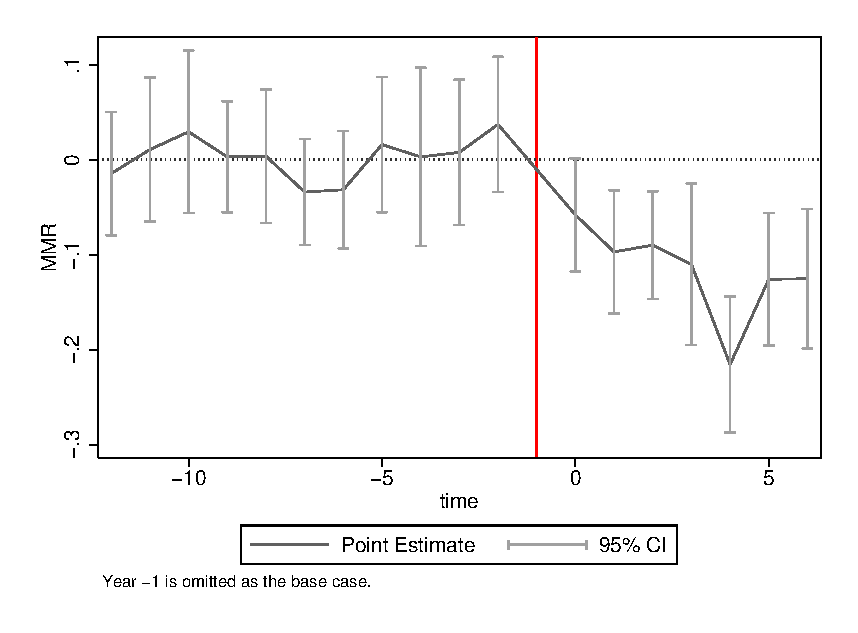
\includegraphics[scale=0.95]{../Source/atheen/eventMMR.eps}
\end{figure}

\begin{figure}[htpb!]
\caption{Pneumonia (Placebo) Event Study Plot}
\label{eventIPR}
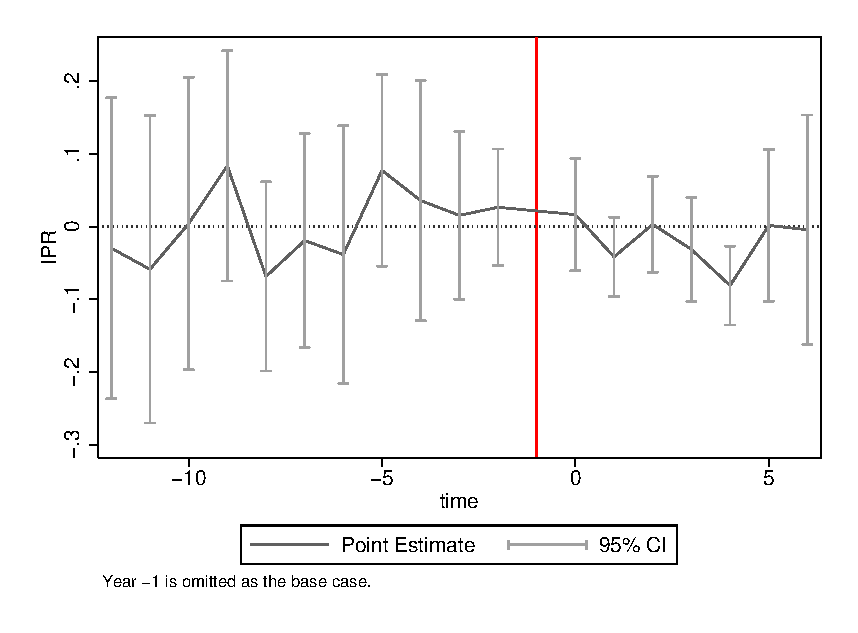
\includegraphics[scale=0.95]{../Source/atheen/eventIPR.eps}
\end{figure}

\newpage
\section*{Tables}
\begin{table}[htbp]\centering
\def\sym#1{\ifmmode^{#1}\else\(^{#1}\)\fi}
\caption{MMR and Desired Sex Ratio (boys/girls)}
\scalebox{0.7}{
\begin{tabular}{l*{5}{c}}
\toprule
                    &\multicolumn{1}{c}{(1)}   &\multicolumn{1}{c}{(2)}   &\multicolumn{1}{c}{(3)}   &\multicolumn{1}{c}{(4)}   &\multicolumn{1}{c}{(5)}   \\
                    &     MMR \ \   &     MMR \ \   &     MMR \ \   &     MMR \ \   &     MMR \ \   \\
\midrule
Desired Sex Ratio   &       824.7** &       655.0** &       667.0** &       923.9***&      2627.7***\\
                    &     [329.4]   &     [299.3]   &     [286.5]   &     [252.9]   &     [617.9]   \\
ln(GDP)             &               &               &        40.9   &        12.4   &       318.5***\\
                    &               &               &      [48.5]   &      [49.8]   &     [119.6]   \\
Desired Sex Ratio$\times$ ln(GDP)&               &               &               &               &      -285.3***\\
                    &               &               &               &               &     [100.7]   \\
Constant            &      -476.0   &      -405.1   &      -712.6   &     -1514.3***&     -3371.0***\\
                    &     [358.9]   &     [325.8]   &     [494.2]   &     [483.9]   &     [734.5]   \\
\midrule
R-squared           &        0.09   &        0.92   &        0.92   &        0.93   &        0.93   \\
Observations        &         310   &         310   &         307   &         307   &         307   \\
 Country FE &&Y&Y&Y&Y\\ Year FE&&Y&Y&Y&Y\\ 
Desired Fertility&&&&Y&Y\\
\bottomrule\end{tabular}}\end{table}

\input{./../Results/dsr/ln_LE_ratio-DSR.tex}
\input{./../Results/dsr/tb-DSR.tex}
\input{./../tables/rightsMMR.tex}
\input{./../tables/rightstb.tex}
\input{./../tables/rightsln_LE_ratio.tex}
\begin{landscape}
\input{./../tables/MMRGII.tex}
\end{landscape}
\begin{landscape}
\input{./../tables/ln_LE_ratioGII.tex}
\end{landscape}
\begin{landscape}
\begin{table}[htbp]\centering
\def\sym#1{\ifmmode^{#1}\else\(^{#1}\)\fi}
\caption{TB and Gender Intensity of Language Measures}
\scalebox{0.5}{
\begin{tabular}{l*{8}{c}}
\toprule
\textsc{Dep Var}:   &\multicolumn{1}{c}{(1)}&\multicolumn{1}{c}{(2)}&\multicolumn{1}{c}{(3)}&\multicolumn{1}{c}{(4)}&\multicolumn{1}{c}{(5)}&\multicolumn{1}{c}{(6)}&\multicolumn{1}{c}{(7)}&\multicolumn{1}{c}{(8)}\\
TB Incidence        &\multicolumn{1}{c}{NGII}&\multicolumn{1}{c}{SBII}&\multicolumn{1}{c}{GPII}&\multicolumn{1}{c}{GAII}&\multicolumn{1}{c}{GII0}&\multicolumn{1}{c}{GII1}&\multicolumn{1}{c}{GII2}&\multicolumn{1}{c}{GTroiano}\\
\midrule
\multicolumn{9}{l}{\textsc{Panel A: No Interaction}}\\
Gender Intensity Index&     -35.418*  &     -38.718   &     -70.779** &      19.500   &      -2.428   &       0.655   &     -23.346** &      -0.365   \\
                    &    [18.025]   &    [26.189]   &    [28.896]   &    [29.072]   &     [7.586]   &     [9.328]   &    [10.351]   &     [4.403]   \\
ln(GDP)             &     -40.202***&     -39.557***&     -49.045***&     -21.397** &     -21.940** &     -21.906** &     -38.367***&     -27.911***\\
                    &    [12.645]   &    [12.493]   &    [14.762]   &    [10.676]   &    [10.279]   &    [10.760]   &    [12.174]   &     [6.210]   \\
R-squared           &        0.55   &        0.55   &        0.52   &        0.58   &        0.57   &        0.57   &        0.56   &        0.55   \\
Observations        &        2619   &        2619   &        2561   &        1893   &        1812   &        1893   &        2469   &        1742   \\
\\ \multicolumn{9}{l}{\textsc{Panel B: GDP Interaction}}\\
Gender Intensity Index&    -113.987   &    -106.469   &    -212.387*  &      49.996   &      -5.372   &       2.209   &     -62.639*  &      15.251   \\
                    &    [80.285]   &    [88.634]   &   [109.688]   &   [151.564]   &    [34.552]   &    [44.033]   &    [36.067]   &    [22.170]   \\
GII $\times$ ln(GDP)&       9.411   &       8.485   &      17.487   &      -3.786   &       0.384   &      -0.204   &       5.032   &      -1.779   \\
                    &     [8.283]   &     [9.232]   &    [12.137]   &    [16.701]   &     [3.870]   &     [5.102]   &     [3.871]   &     [2.310]   \\
ln(GDP)             &     -44.724***&     -45.505***&     -54.743***&     -18.746   &     -22.978   &     -21.476   &     -46.338***&     -23.369***\\
                    &    [14.407]   &    [16.554]   &    [16.091]   &    [16.231]   &    [14.999]   &    [15.856]   &    [15.425]   &     [8.129]   \\
\midrule
R-squared           &        0.56   &        0.55   &        0.52   &        0.58   &        0.57   &        0.57   &        0.56   &        0.55   \\
Observations        &        2619   &        2619   &        2561   &        1893   &        1812   &        1893   &        2469   &        1742   \\
\bottomrule 
\end{tabular}}\end{table}

\end{landscape}
\input{./../tables/mechanism.tex}


\newpage
\section*{Appendix Tables}
\input{./../Results/rights/MMR-WP.tex}
\input{./../Results/rights/ln_LE_ratio-WP.tex}
\input{./../Results/rights/tb-WP.tex}


\end{spacing}
\end{document}



*POINT 1: 
